\section{Results}\label{sec:results}
% Write this section FIRST. Use the macros (e.g. \CoalDkFour) instead of typing numbers.

\subsection{Insider-coalition exposure}
\begin{figure}[t]
\centering
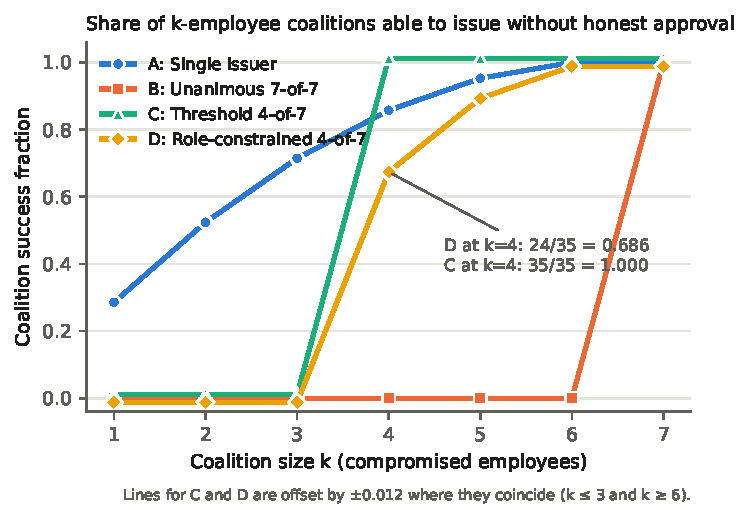
\includegraphics[width=\columnwidth]{fig_coalition}
\caption{Fraction of $k$-employee coalitions able to issue a credential without any honest approval.}
\label{fig:coalition}
\end{figure}

\begin{figure*}[t]
\centering
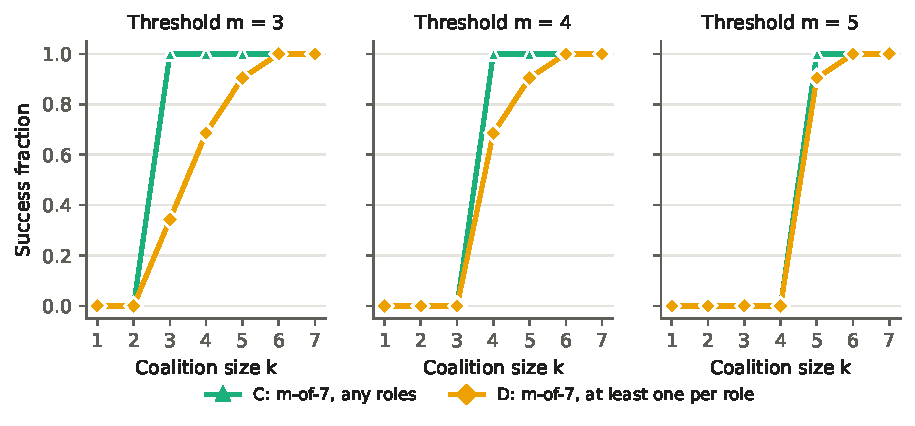
\includegraphics[width=0.85\textwidth]{fig_coalition_sensitivity}
\caption{Threshold policy (C) versus role-constrained policy (D) at thresholds 3, 4 and 5.}
\label{fig:coalition-sensitivity}
\end{figure*}

% Generated by experiments/generate_figures.py -- do not edit by hand.
\begin{table*}[t]
\centering
\small
\caption{Coalitions of $k$ employees able to issue, per policy (2 Registrars, 3 Deans, 2 Exam Officers).}
\label{tab:coalition}
\begin{tabular}{crrrr}
\hline
$k$ & A & B & C (4-of-7) & D (4-of-7, roles) \\
\hline
1 & 2/7 (0.286) & 0/7 (0.000) & 0/7 (0.000) & 0/7 (0.000) \\
2 & 11/21 (0.524) & 0/21 (0.000) & 0/21 (0.000) & 0/21 (0.000) \\
3 & 25/35 (0.714) & 0/35 (0.000) & 0/35 (0.000) & 0/35 (0.000) \\
4 & 30/35 (0.857) & 0/35 (0.000) & 35/35 (1.000) & 24/35 (0.686) \\
5 & 20/21 (0.952) & 0/21 (0.000) & 21/21 (1.000) & 19/21 (0.905) \\
6 & 7/7 (1.000) & 0/7 (0.000) & 7/7 (1.000) & 7/7 (1.000) \\
7 & 1/1 (1.000) & 1/1 (1.000) & 1/1 (1.000) & 1/1 (1.000) \\
\hline
\end{tabular}
\end{table*}


\note{Key facts to explain in your own words. Under A, a single insider suffices (\CoalAkOne{} of the single
employees). At threshold 4, role constraints leave the minimum coalition size unchanged (4) but reduce capable
4-person coalitions from \CoalCkFour{} to \CoalDkFour{} (\CoalDkFourFrac). The effect is larger at threshold 3
(\CoalCthreekThree{} vs.\ \CoalDthreekThree) and nearly vanishes at 5 (\CoalCfivekFive{} vs.\
\CoalDfivekFive). Why: with more required approvers, almost every coalition already spans all roles.}

\subsection{Gas consumption}
\begin{figure}[t]
\centering
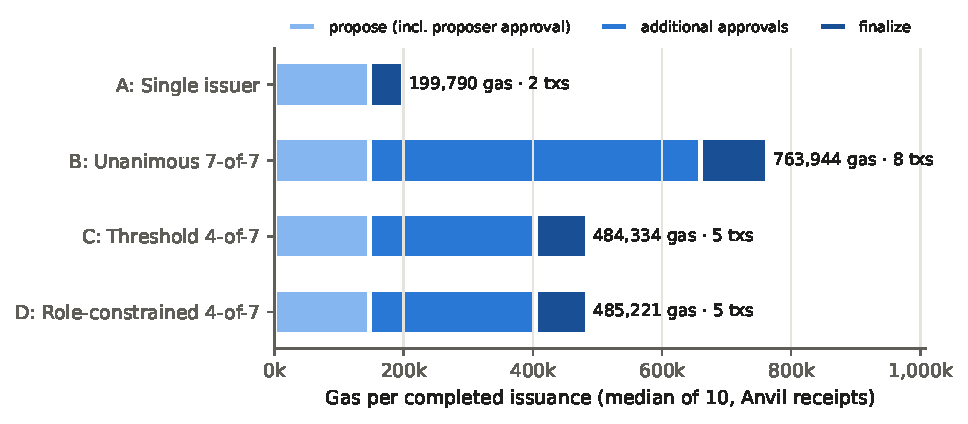
\includegraphics[width=\columnwidth]{fig_gas}
\caption{Gas per completed issuance (median of 10), split into proposal, additional approvals and finalization.}
\label{fig:gas}
\end{figure}

% Generated by experiments/generate_figures.py -- do not edit by hand.
\begin{table*}[t]
\centering
\small
\caption{Median gas from Anvil transaction receipts (10 issuances per policy).}
\label{tab:gas}
\begin{tabular}{lrrrr}
\hline
Operation & A & B & C & D \\
\hline
Deploy policy & 150,365 & 153,379 & 170,266 & 286,817 \\
Deploy registry & 2,615,457 & 2,615,457 & 2,615,457 & 2,615,457 \\
Add approver & 65,495 & 65,495 & 65,495 & 65,495 \\
Change role & 43,930 & 43,930 & 43,930 & 43,930 \\
(De)activate approver & 37,809 & 37,809 & 37,809 & 37,809 \\
Propose & 146,228 & 146,231 & 146,253 & 146,253 \\
Approve (each) & -- & 85,639 & 85,661 & 85,661 \\
Finalize & 53,562 & 103,879 & 81,098 & 81,985 \\
Revoke & 54,501 & 54,501 & 54,501 & 54,501 \\
Verify (eth\_call estimate) & 29,408 & 29,408 & 29,408 & 29,408 \\
\textbf{Total per issuance} & \textbf{199,790} & \textbf{763,944} & \textbf{484,334} & \textbf{485,221} \\
Transactions per issuance & 2 & 8 & 5 & 5 \\
\hline
\end{tabular}
\end{table*}


\note{Totals: A \GasTotalA, B \GasTotalB, C \GasTotalC, D \GasTotalD{} gas. The role check costs
\GasRoleOverhead{} gas (\GasRoleOverheadPct) per issuance, all in finalization (\GasFinalizeC{} vs.\
\GasFinalizeD). Cost scales with the number of approvals (\GasApproveEach{} gas each), not with the policy
logic.}

\subsection{Availability and delay}
\begin{figure*}[t]
\centering
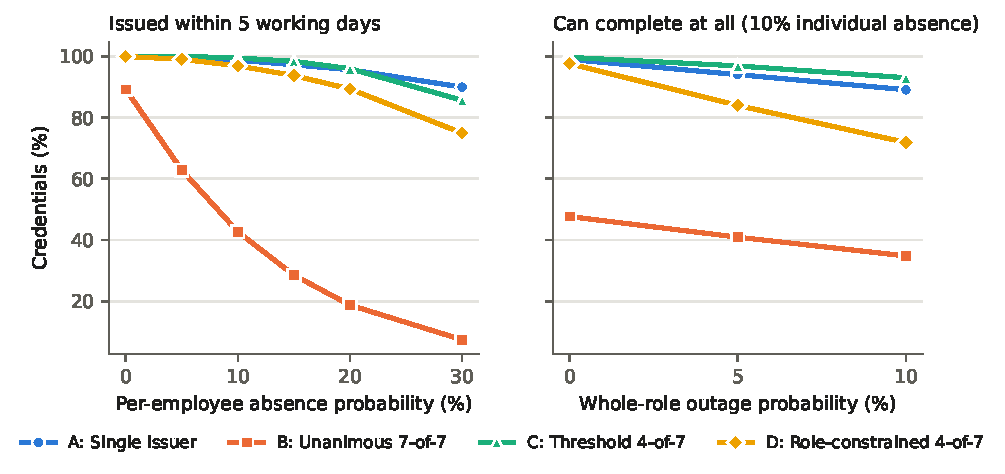
\includegraphics[width=0.85\textwidth]{fig_availability}
\caption{Left: credentials issued within 5 working days versus individual absence. Right: credentials that can
be issued at all versus the probability that an entire role is unavailable (10\% individual absence).
Simulated.}
\label{fig:availability}
\end{figure*}

\begin{figure*}[t]
\centering
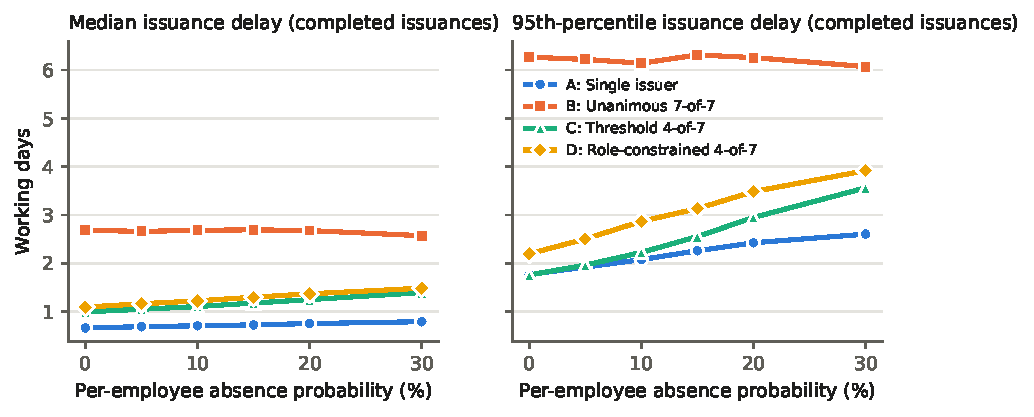
\includegraphics[width=0.85\textwidth]{fig_delay}
\caption{Median and 95th-percentile simulated issuance delay of completed issuances.}
\label{fig:delay}
\end{figure*}

% Generated by experiments/generate_figures.py -- do not edit by hand.
\begin{table}[t]
\centering
\small
\caption{Simulated workflow at 10\% individual absence (20{,}000 trials, seed 435, deadline 5 working days). Delays in working days over completed issuances.}
\label{tab:availability}
\begin{tabular}{lrrrrrr}
\hline
Policy & Completes & On time & Median & P95 & Cannot complete & of which: role \\
\hline
A: Single issuer & 99.0\% & 98.7\% & 0.71 & 2.08 & 1.0\% & 1.0\% \\
B: Unanimous 7-of-7 & 47.7\% & 42.7\% & 2.68 & 6.14 & 52.3\% & 0.0\% \\
C: Threshold 4-of-7 & 99.6\% & 99.5\% & 1.10 & 2.22 & 0.4\% & 0.0\% \\
D: Role-constrained 4-of-7 & 97.6\% & 96.9\% & 1.22 & 2.87 & 2.4\% & 2.1\% \\
\hline
\end{tabular}
\end{table}


\note{At 10\% absence, on-time issuance is A \OnTimeA, B \OnTimeB, C \OnTimeC, D \OnTimeD. D's extra failures
are caused by a missing role (\MissingRoleD{} of trials). Under a 5\% whole-role outage, D completes
\OutageFiveD{} versus \OutageFiveC{} for C (at 10\%: \OutageTenD{} versus \OutageTenC). Unanimous is
impractical (\CompleteB{} completion).}

\subsection{Security--cost--availability trade-off}
\begin{figure}[t]
\centering
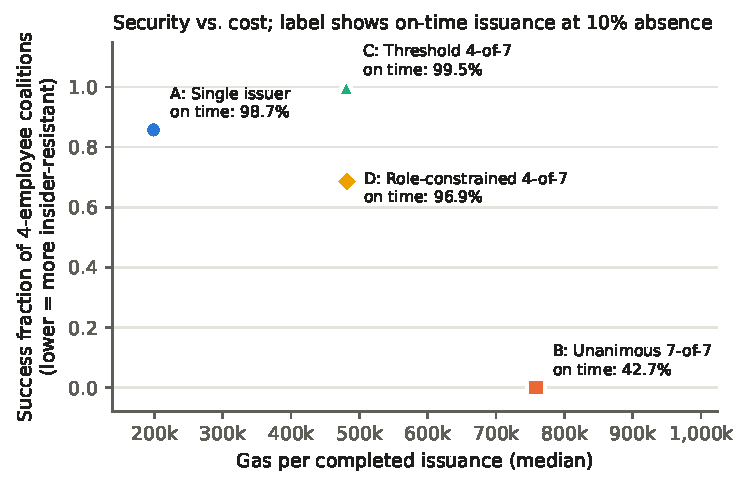
\includegraphics[width=\columnwidth]{fig_tradeoff}
\caption{Coalition exposure at $k=4$ versus gas per issuance; labels give on-time issuance at 10\% absence.}
\label{fig:tradeoff}
\end{figure}
\note{One paragraph that answers the research question directly. No policy dominates on all three axes.}
